\chapter{評価と考察}
\label{eval}

本章では,予備実験と\ref{impl}章で実装した本研究での提案手法の評価とその考察を述べる.

\section{予備実験}
\label{eval:first}

%\subsection{概要}
%\label{eval:abst}
SSHの低対話型HoneypotであるCowrieはコマンドの実装数が少なく,Cowrie特有の異常な挙動が多い.そのため,侵入者にHoneypotであると検知されることで,本来実際のOSへの攻撃であれば取れるはずであった侵入ログが取れない問題がある.また,収集ログを分析する際に,これまで用いられてきた"危険なコマンド"としてインデックスを作り,それらを危険なコマンドとしてパターンマッチングする手法では,今後出現してくる様々なコマンドパターンなどに対応できない.\\
予備実験では,Cowrieはコマンドの実装数が少なく,Cowrie特有の異常な挙動が多いため,コマンドの追加実装を行い,Cowrie特有の異常な挙動を修正した.実装を施していない純正のCowrieとCowrieにBusyBoxに含まれるコマンドを実装した修正済みのCowrieの両方でコマンドログの収集を行い,比較することで,収集ログのパターンの変化を観測できるのではないかと考えた.評価として収集した二つのログをSkip-gramモデルを用いてスコアリングし,どちらがより多くのコマンドログのパターンを収集できているのかを検証した.\\
その結果,より多くのコマンドパターンを取れたのがCowrieにBusyBoxに含まれるコマンドを実装した修正済みのCowrieであるということが明らかとなった.

\subsection{予備実験の手法}
\label{eval:appr}
実装を施していない純正のCowrieに対して,これには実装されていないがShellには実装されているコマンドを実装したものを設置し,ログを収集した.

\subsection{侵入ログの収集環境}
\label{eval:apprenv}


\subsection{実装}
\label{eval:impl}
純正のCowrieにBusyBoxに含まれるコマンドを実装し,またHoneypot特有の異常な挙動を修正した.ここでの実装を紹介する.

\subsection{評価}
\label{eval:eval}
実装を施していない純正のCowrieとCowrieにBusyBoxに含まれるコマンドを実装した修正済みのCowrieの両方で侵入ログの収集を行い,Word2vecのSkip-Gram Modelにより次のコマンドの予測,スコアリングを行い比較を行うことで,差異を評価した.スコアリングでは,あるコマンドが実行された時に次のコマンドの出やすさを予測したため,次に実行されるコマンドがスコアとして高い数値を出せばそのコマンドパターンがパターンとして存在しやすいものであることを示す.予備実験の評価に関しては第7章の評価で一部説明している.
本研究の評価と評価手法の違いは,モデル化を純正のHoneypotにBusyBoxに含まれるコマンドを実装したものしか行っていないため,実際のOSに近いログが取れたことが証明できておらず,比較する対象が少なかった.

\subsection{結果}
\label{eval:conc}
SSHの低対話型Honeypotの稼働期間は12/10から2/1(54日間)で,収集できたものとしてコネクション数,パターン数,コマンド数を以下の図6.1に記す.

\begin{figure}[H]
    \centering
    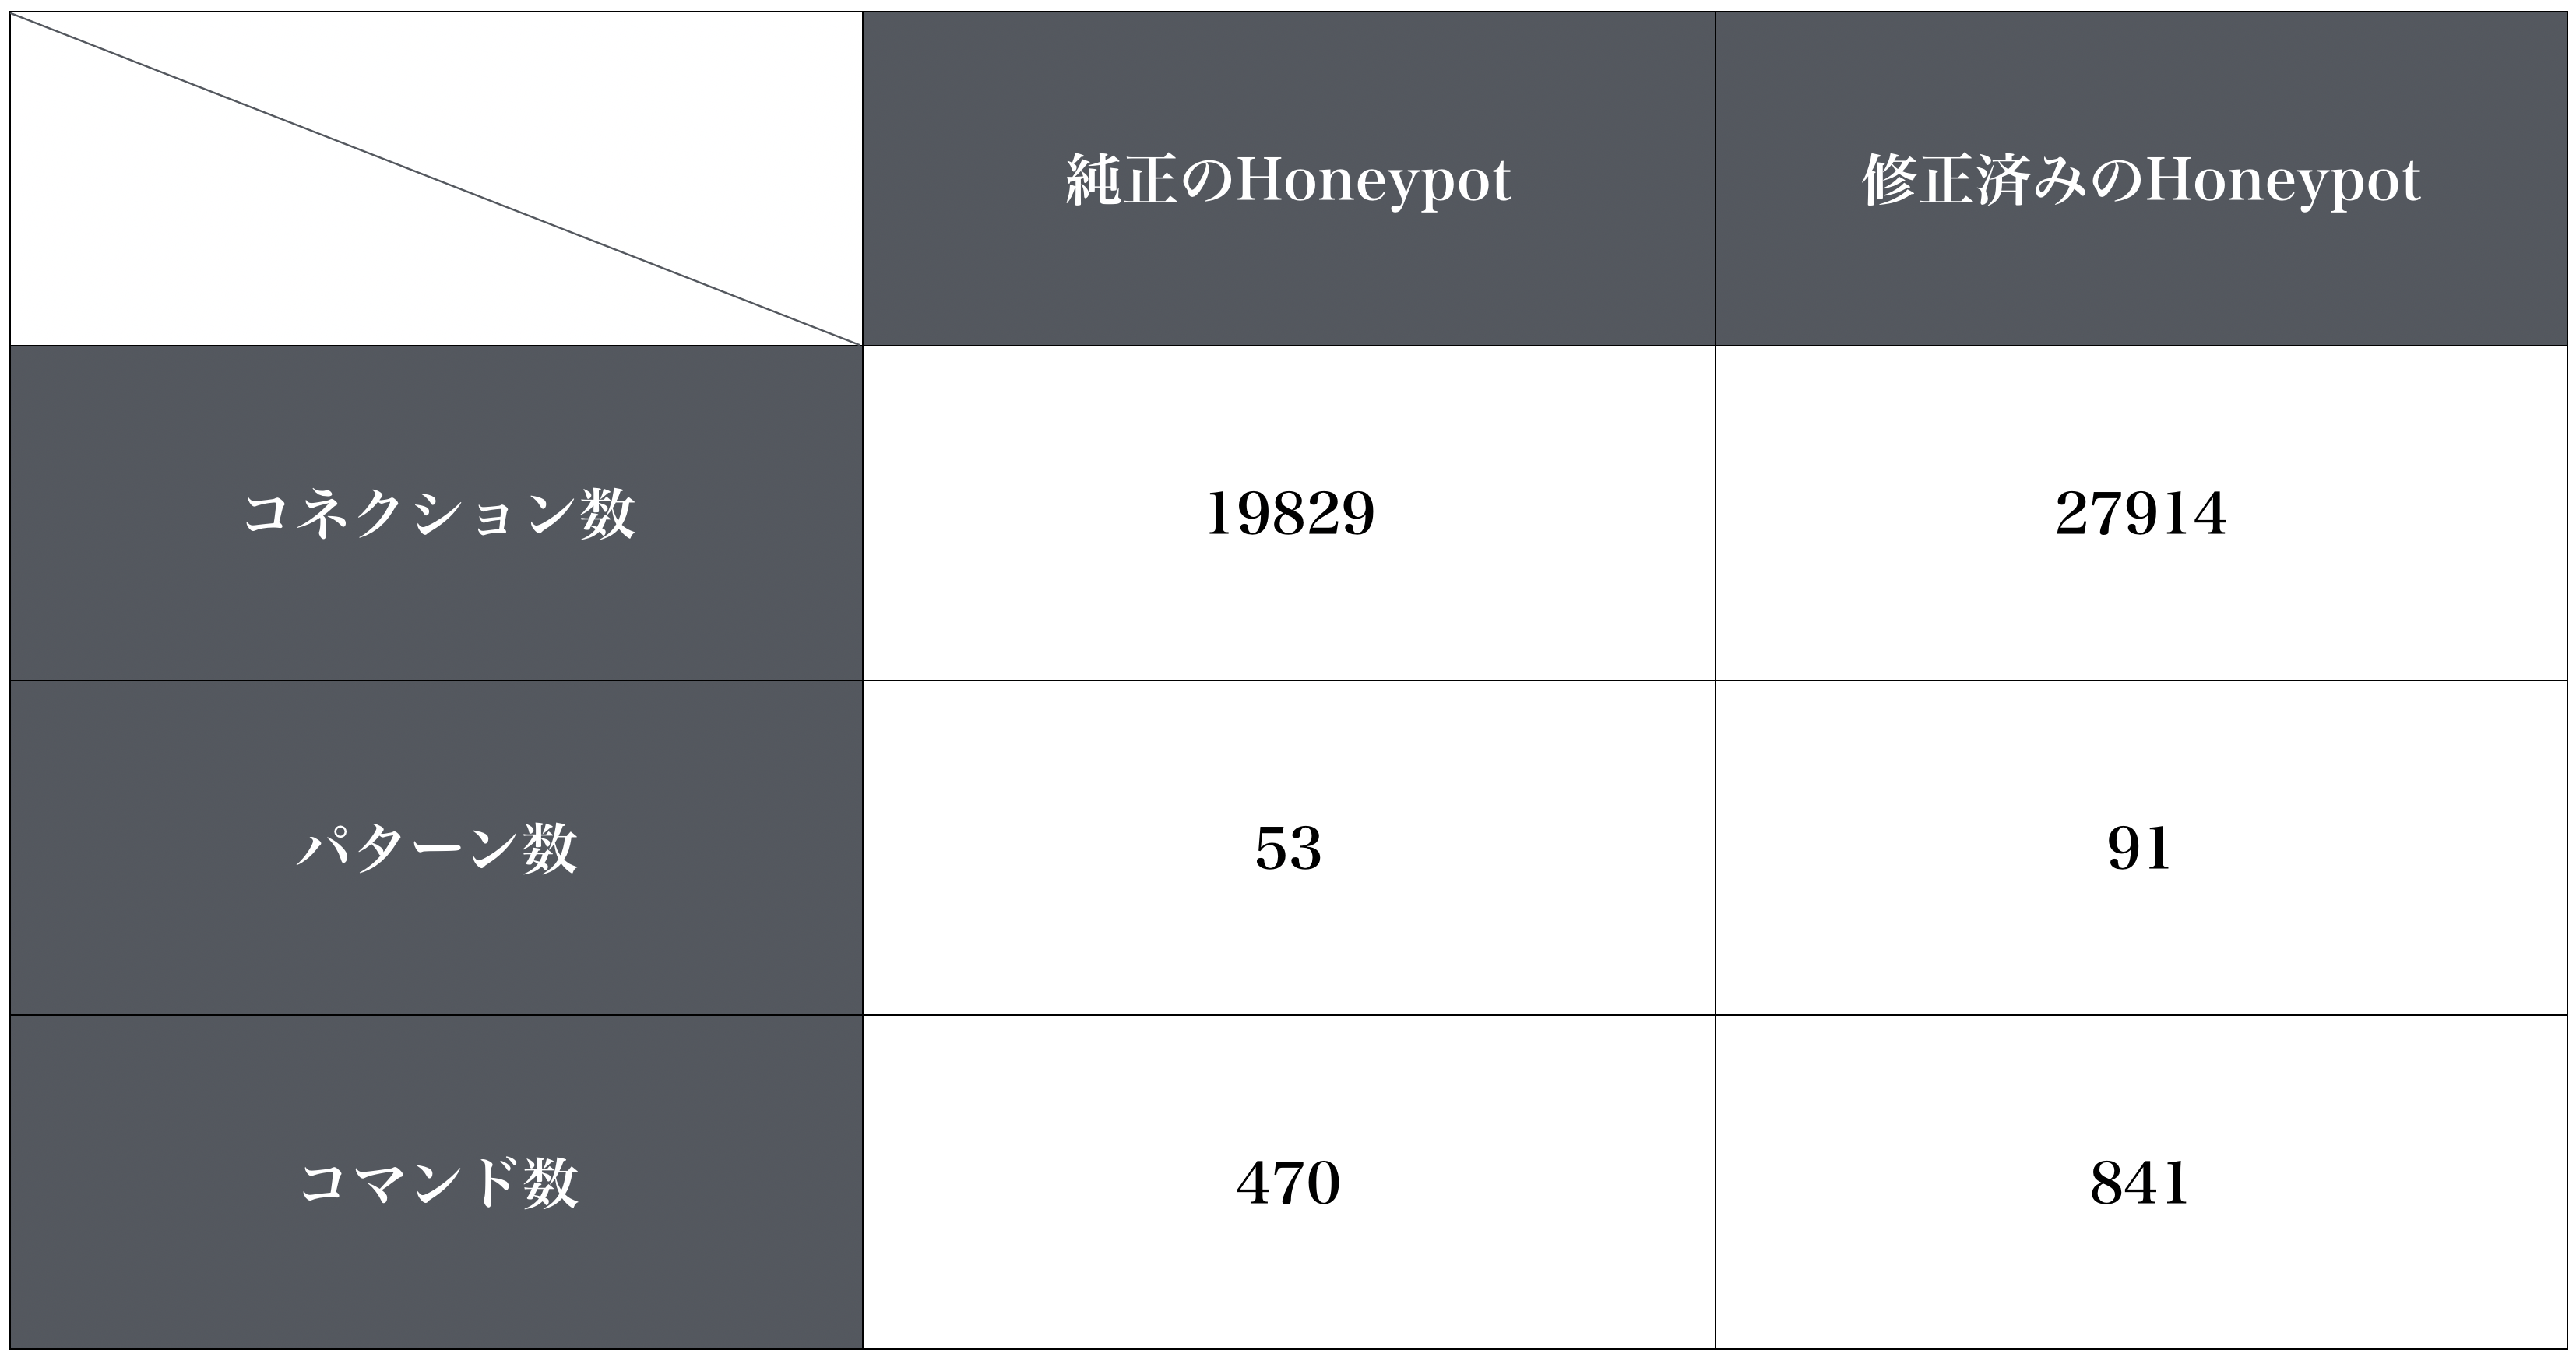
\includegraphics[width=1.0\textwidth]{figures/term.png}
    \caption{収集したSSHの低対話型Honeypotのデータ}
    \label{fig:evo}
\end{figure}

また,モデル化を行い純正のCowrieとCowrieにBusyBoxに含まれるコマンドを実装した修正済みのCowrieのスコアリングを行なった結果を以下の図6.2に記す.横軸はコマンド拡張を行なったHoneypotか素のHoneypotであるかを示している.縦軸は予備実験の評価手法によって算出されたコマンドの表れやすさを数値化したものであり,数値が高くなればのコマンドパターンがパターンとして存在しやすいものであることを示している.予備実験ではコマンドの拡張実装をしたものの方がコマンドパターンとして存在しにくいものを観測できたという結果になった.

\begin{figure}[H]
    \centering
    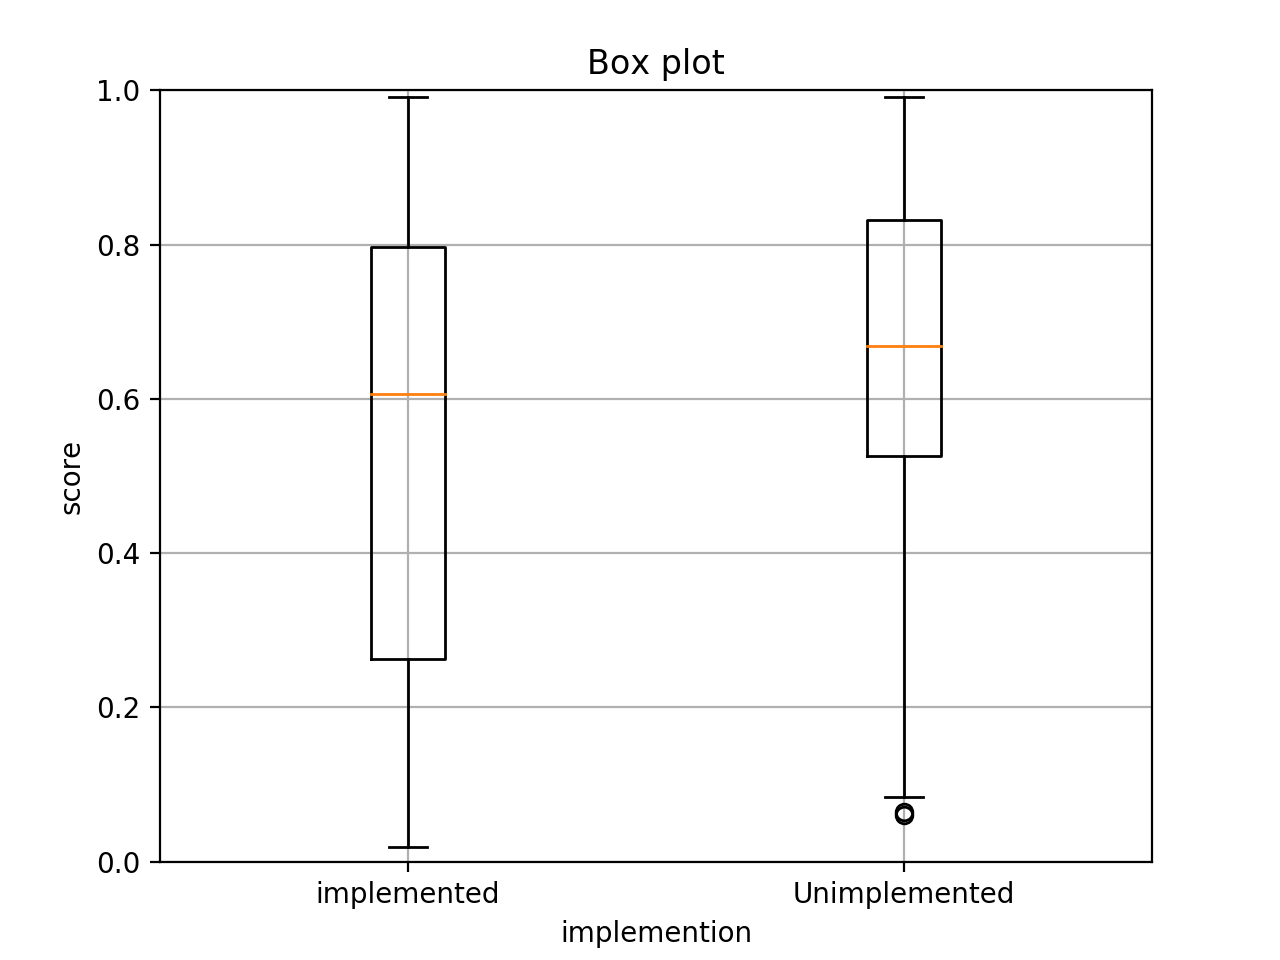
\includegraphics[width=1.0\textwidth]{figures/Figure_1.png}
    \caption{純正のCowrieと修正済みのCowrieのスコアリングによる比較}
    \label{fig:evo}
\end{figure}

本研究の予備実験では,Cowrieに実装されていないコマンドで悪意のある侵入者が使うようなコマンドを実装し,何の追加実装も施していないCowrieで取れた侵入者の実行コマンドログと ,追加実装を施したCowrieの侵入者の実行コマンドログを比較することで,追加実装を施したSSHのCowrieの方がコマンドパターンとして多く収集できることを示した.


\section{評価手法}
\label{eval:eval}

本研究の仮説の検証手法としての評価として,~\ref{appr:YotenForProblem}節で述べた要件に対して評価を行う.\\
予備実験では,素の低対話型Honeypotよりも,コマンドを拡張したHoneypotの方がコマンドパターンが多く収集できることを示した.本研究では拡張したHoneypotで収集したコマンドログが,どれほど高対話型Honeypotで収集したコマンドログに近似したのかを評価した.\\
本研究では,以下の三種類のHoneypotを設置する.\\
1. 広く利用されているSSHの低対話型Honeypot\\
2. 実際のShellには実装されているが,1.のHoneypotで未実装のコマンドを実装したHoneypot\\
3. 広く利用されている高対話型Honeypot\\

これ以降,1.の広く利用されているSSHの低対話型Honeypotのことを”純正の低対話型Honeypot” , 2.の実際のShellには実装されているが,1.のHoneypotで未実装のコマンドを実装したHoneypotのことを"修正済みの低対話型Honeypot" , 3.の広く利用されている高対話型Honeypotのことを"高対話型Honeypot"と呼ぶこととする.\\

%以上3つの純正のHoneypot,修正済みのHoneypot,高対話型Honneypotのそれぞれで侵入ログを収集する.\\

また予備実験では,純正のHoneypotに実装されていないコマンドで悪意のある侵入者が使うようなコマンドを実装し,純正のHoneypotで取れた侵入者の実行コマンドログと,修正済みのHoneypotの侵入者の実行コマンドログを比較することで,修正済みのHoneypotの方がコマンドパターンとして多く収集できることを示した.予備実験における収集ログの比較の概念図を図6.3に示す.

\begin{figure}[H]
    \centering
    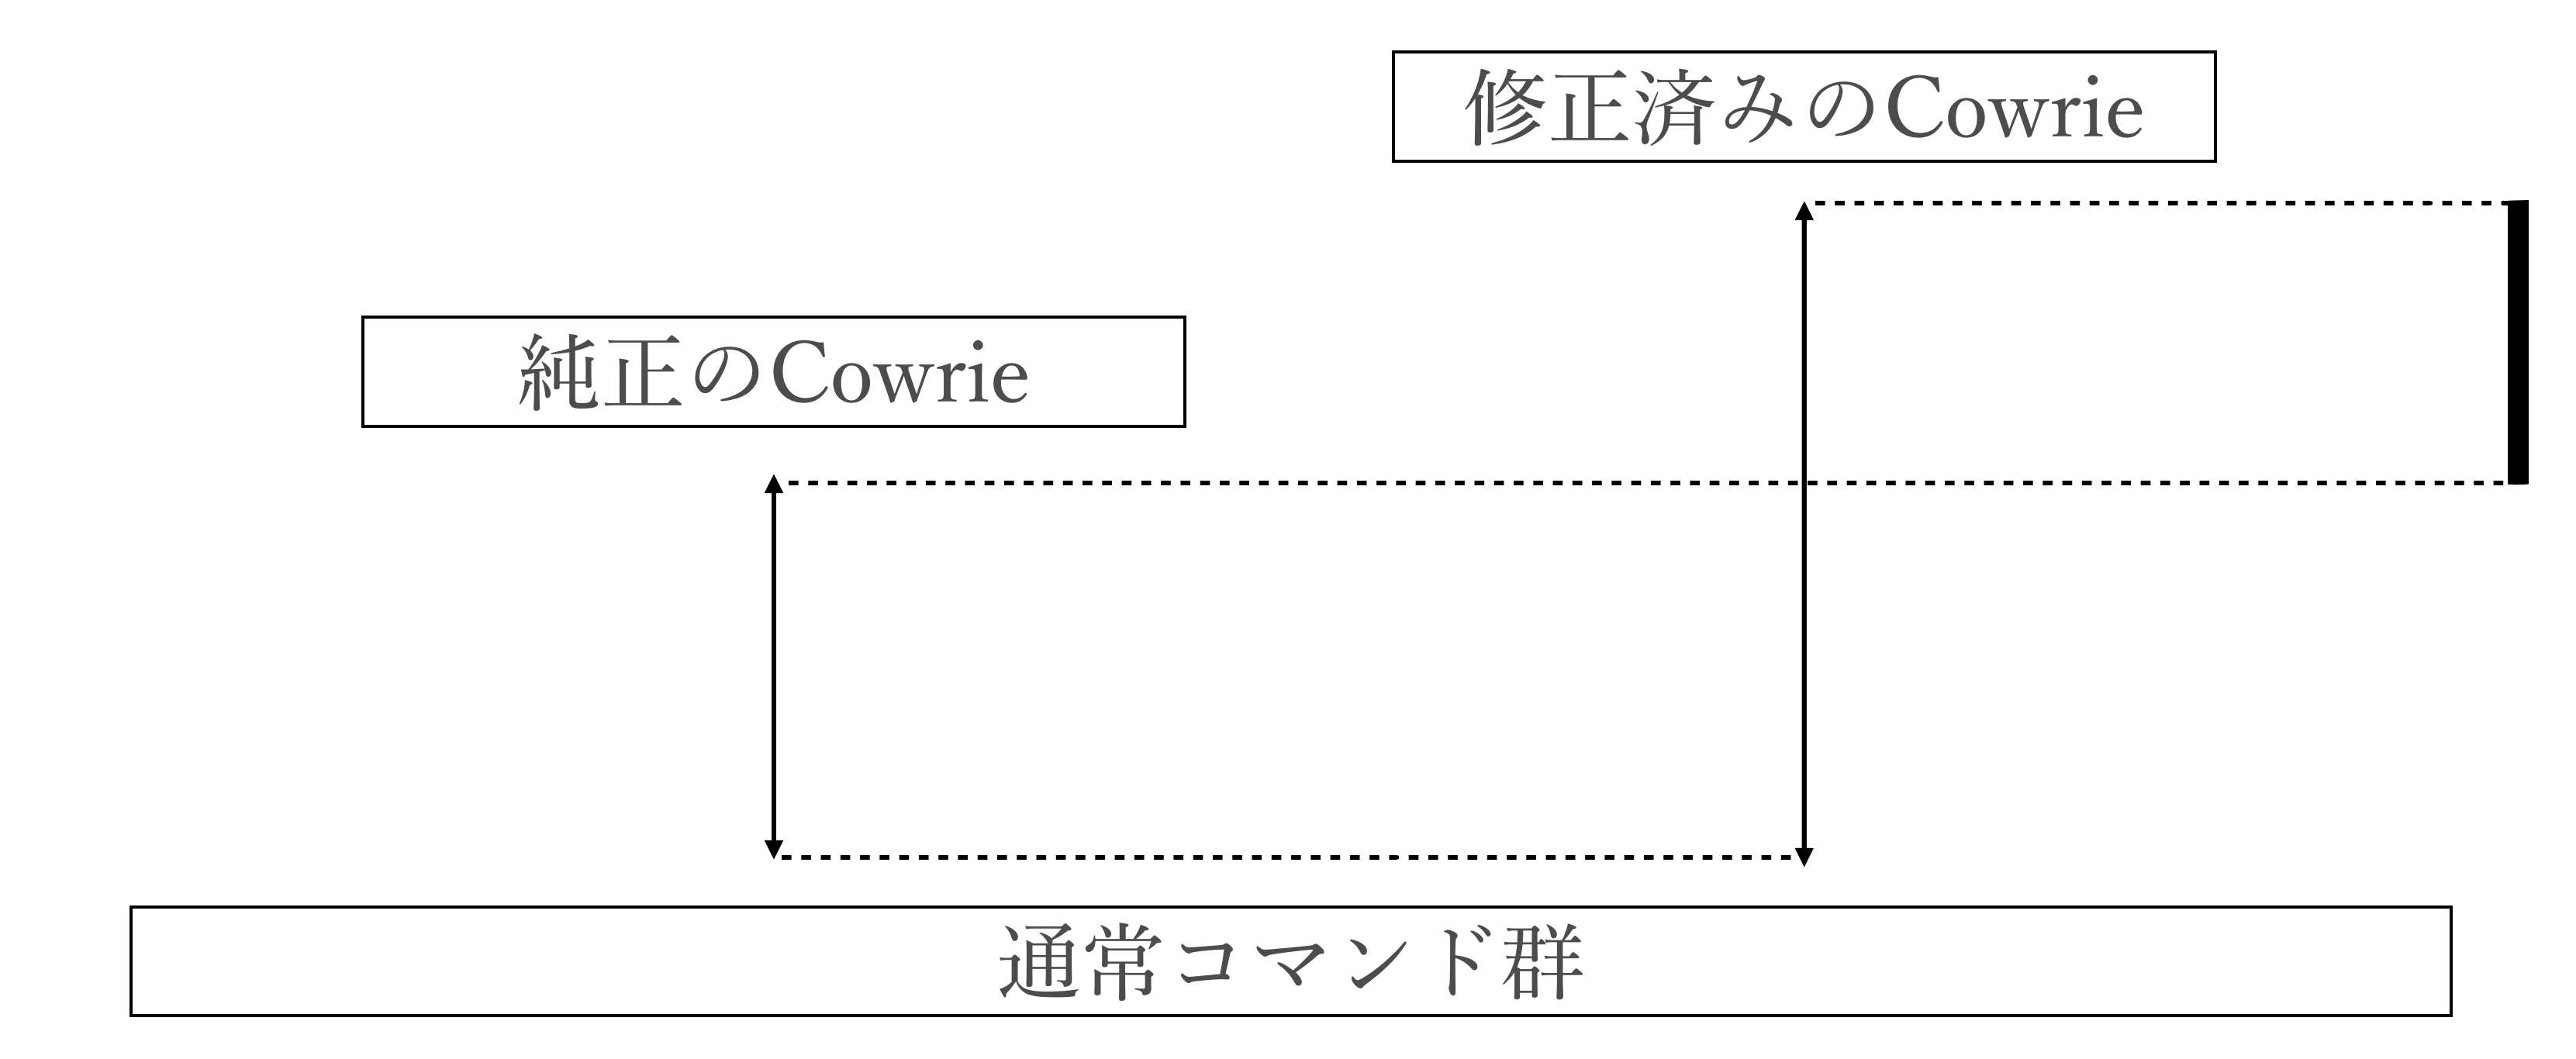
\includegraphics[width=1.0\textwidth]{figures/termhyoka.png}
    \caption{予備実験の評価の概念図}
    \label{fig:evo}
\end{figure}

この予備実験では評価として何の追加実装も施していないSSHの低対話型Honeypotで取れた侵入者の実行コマンドログと追加実装を施したSSHの低対話型Honeypotの侵入者の実行コマンドログとを比較したのに対して,本件研究の評価手法では,純正のHoneypotで取れた侵入者の実行コマンドログと修正済みのHoneypotの侵入者の実行コマンドログをと高対話型Honeypotの侵入者の実行コマンドログを比較することで,修正済みのHoneypotの侵入者の実行コマンドログが実際のShellの挙動にどれほど近似したのかを評価した.予備実験における収集ログの比較の概念図を図6.4に示す.

\begin{figure}[H]
    \centering
    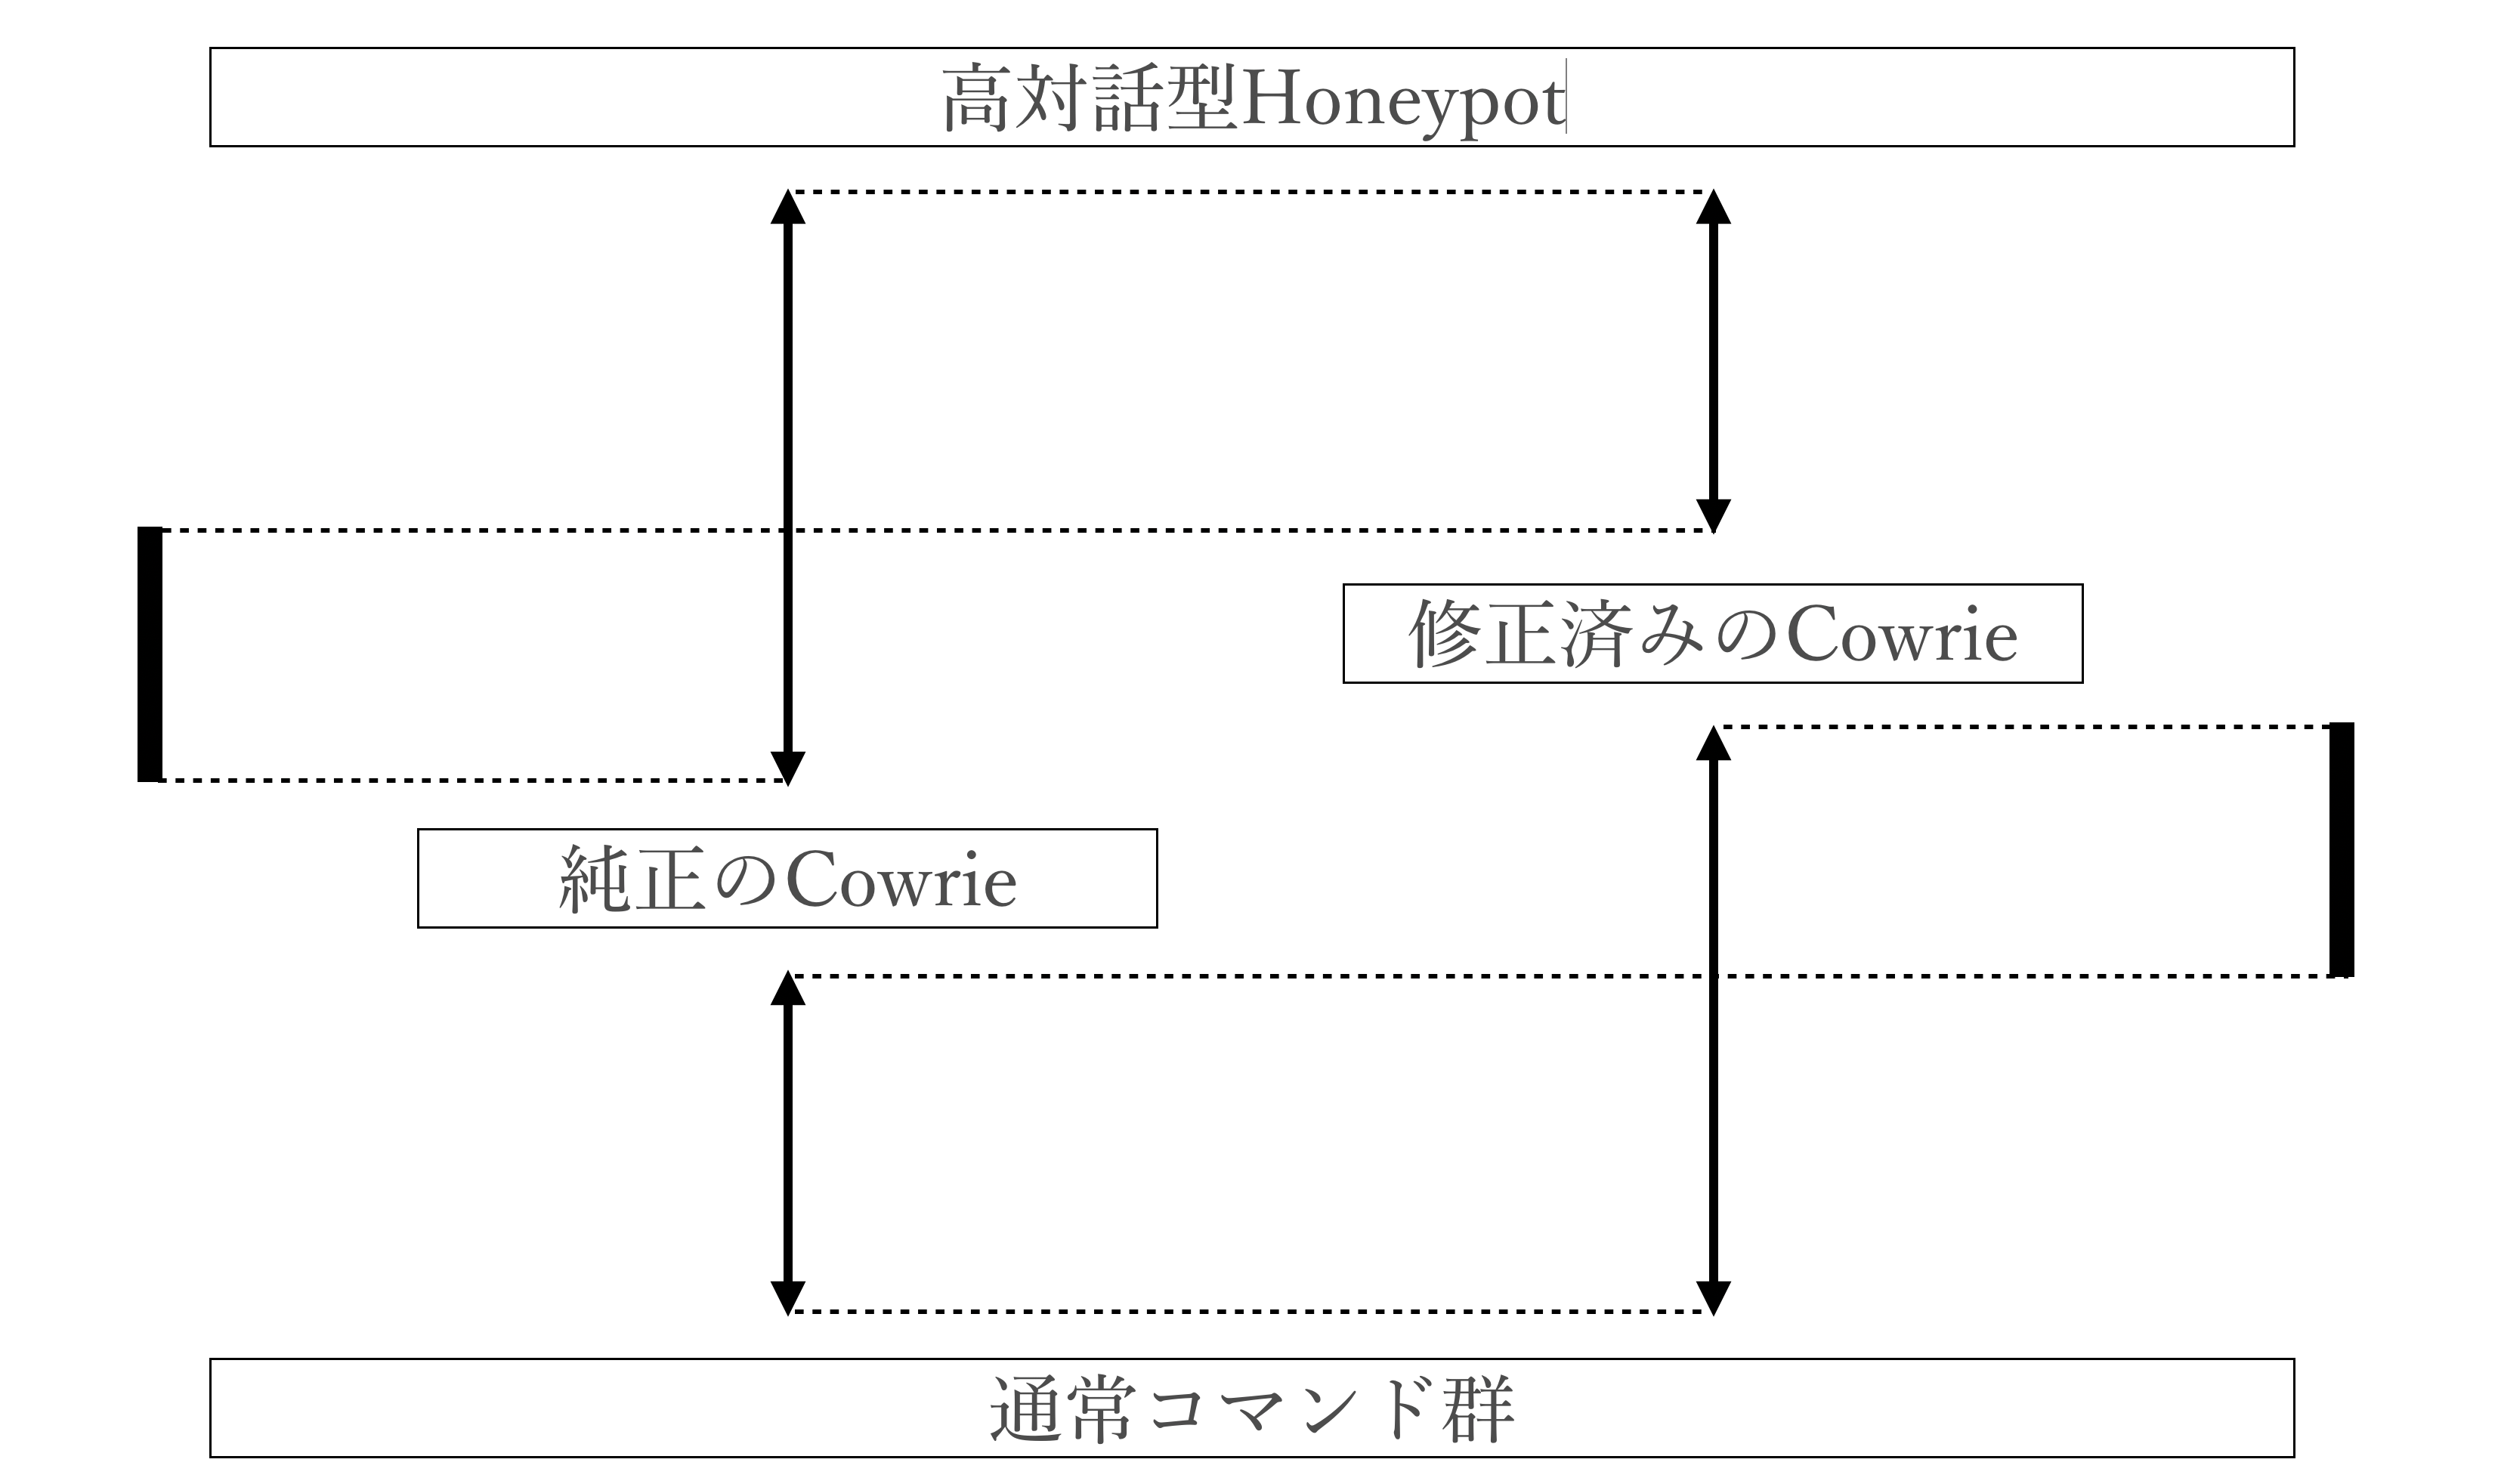
\includegraphics[width=1.0\textwidth]{figures/sotuhyoka.png}
    \caption{本研究の評価の概念図}
    \label{fig:evo}
\end{figure}

%図6,と図7で示したように,取れた収集ログを比較することでいかに高対話型Honeypotに近似できたのか検証する.


\subsection{コマンドログのスコアリング手法の実装の提案}
\label{eval:implsuge}
コマンドログの比較を行う手法は多く存在する.例えば評価基準として,あるコマンドが実行された時に,そのコマンドは危険であるとしたブラックリストを作成するパターンマッチングの手法がある.また,攻撃であるとされたコマンドを~\ref{tech:Markov}で説明したマルコフモデルで学習させることで,攻撃性を表現する手法がある.
しかしパターンマッチングであれば静的解析であるので未知の攻撃に対応ができず,マルコフモデルであれば現在の状態だけに依存して次の状態への推移確率が決まるので,未知の特徴量を無視してしまうので,いずれも未知の攻撃に対応できない.
しかし,~\ref{tech:tokei}で説明した意味解析をコマンドログに導入することで,コマンド名が別でも同じような内容のコマンドを実行しようとした時に,それが同じような内容であることを検知できる自然言語処理における意味解析のニューラルネットワークのモデルを評価基準とすることで未知の攻撃にも対応できる.
そのため,本研究では自然言語処理における意味解析のニューラルネットワークのモデルを評価基準とした.

\subsection{機械学習を用いたコマンドログのスコアリング}
\label{eval:impl}
本研究では,評価基準となる,自然言語処理における意味解析のニューラルネットワークのモデルとしてWord2vecのskip-gramモデルを採用した.
純正の低対話型Honeypotで収集した侵入ログでskip-gramモデルの隠れ層の重みを学習させ(これをモデル1
とする),同様にして高対話型Honeypotで収集した侵入ログもskip-gramモデルの隠れ層の重みを学習させる(これをモデル2とする).次に修正済みのHoneypotで収集したログをセッション開始からセッション終了までに打たれたコマンドごとに(以降これを1セッションごとと呼ぶ)モデル1とモデル2のそれぞれに入力していき,出力された数値aを活性化関数としてソフトマックス関数をかけることで,0≦a≦1の範囲を取るようにし確率的な数値として出力することでスコアリングを行う.このため入力に対して多数存在する出力を全てを合計すると1になる.
純正の低対話型Honeypotや高対話型Honeypotの収集ログをモデル化する際、入力層として収集ログのコマンドの入力に対してそのコマンドの周辺のコマンドを出力として与えることでこれを学習させる.\\
例えば3つのコマンドが打たれたとしたとしたものを以下のプログラム\,6.1に示す.

\vspace{5mm}
%\lstnewenvironment{mylisting}[1][]
%    {\lstset{
%        frame=single,
%        basicstyle=\ttfamily,
%        numbers=left,
%        numbersep=10pt,
%        tabsize=2,
%        extendedchars=true,
%        xleftmargin=17pt,
%        framexleftmargin=17pt,
%        #1
%    }
%}{}

\begin{mylisting}[language=sh,caption=3つの実行コマンドの例]
 $ uname
 $ free
 $ ps x
\end{mylisting}
\vspace{5mm}

モデルを構築する際には"free"コマンドを入力にした時に,出力として"uname"コマンド"ps"コマンドを用意しておくことで,freeが入力として与えられた時に他2つの出力される周辺のコマンドが出力する確率が高くなるようにする.また,実装としては周辺語をどこまで広げるのかはパラメータとしてwindow sizeで与えることができ,上記の例の周辺語は"1"であり,window sizeを"2"にすればモデル化する際に出力層に与えられる数は4つとなる.

以下の図6.5にモデル化のフローを示す.
\vspace{10mm}
\begin{figure}[H]
    \centering
    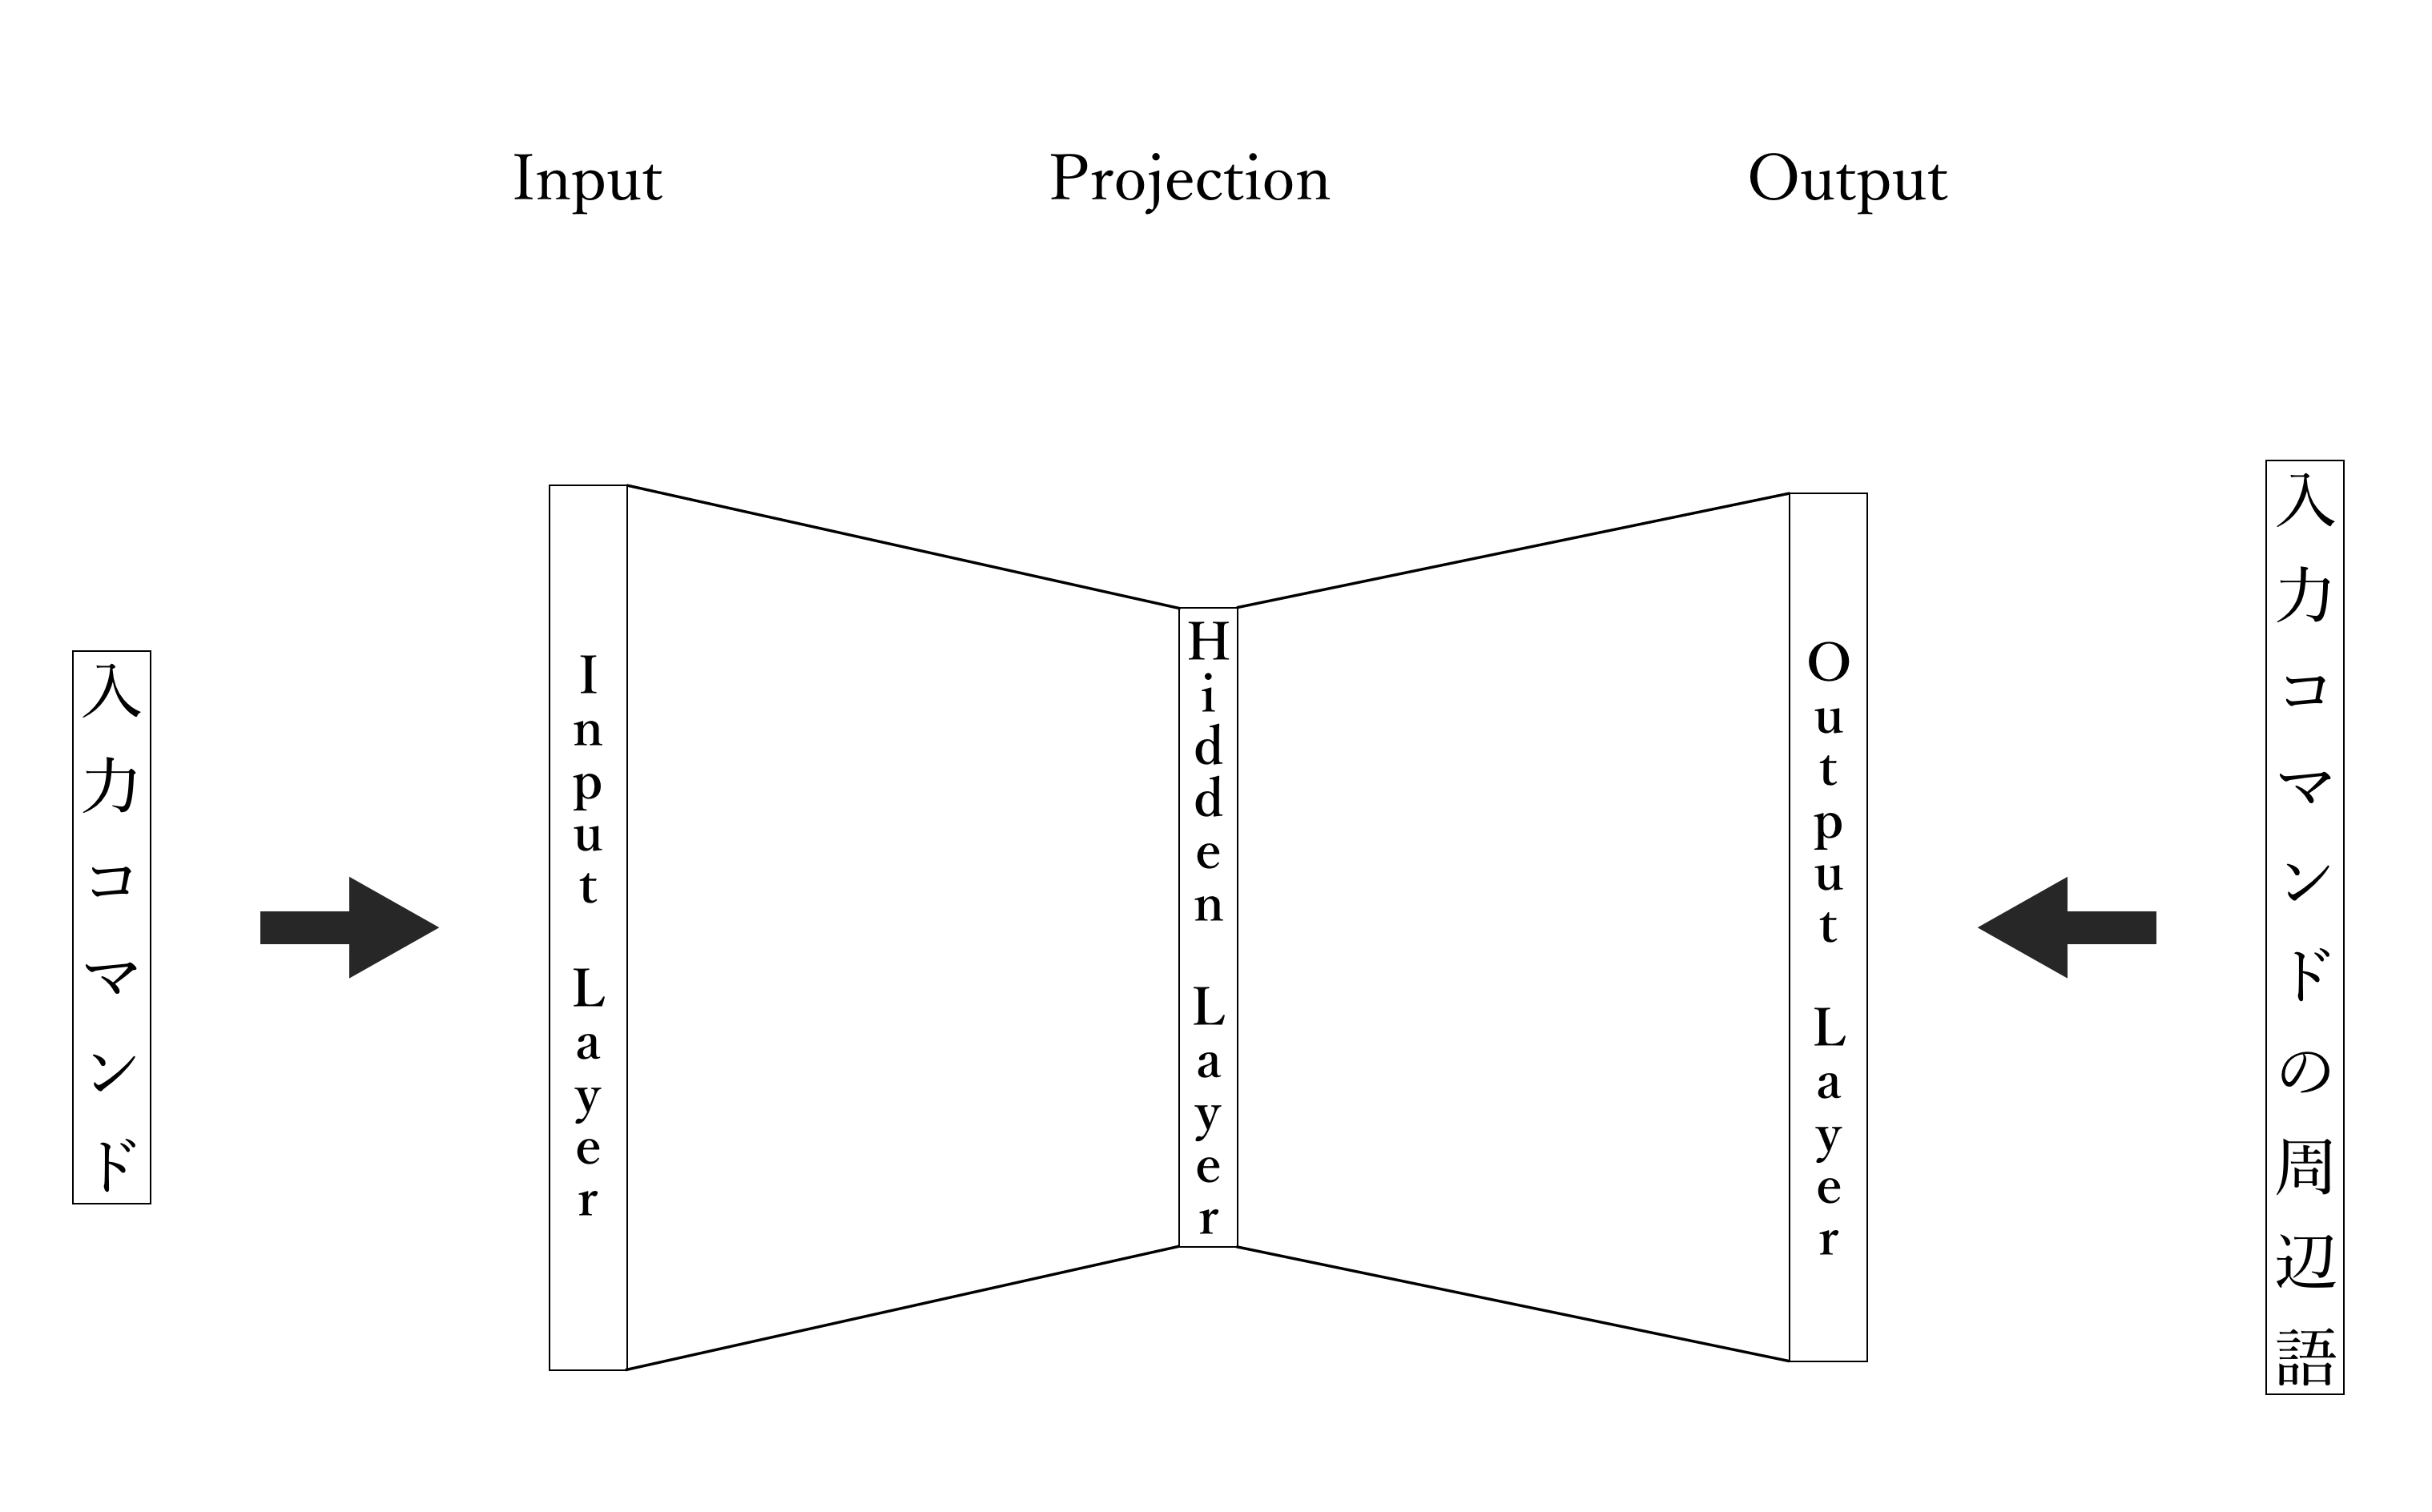
\includegraphics[width=1.0\textwidth]{figures/model.png}
    \caption{評価のフロー\cite{word2vecpaper}\cite{word2vecpaper2}}
    \label{fig:evo}
\end{figure}
\vspace{10mm}
また,このようにして純正の低対話型Honeypotの収集ログと高対話型Honeypotの収集ログに対して各々のモデルを構築する.次にこのモデルに対して,修正済みのHoneypotで収集したログを入力して,確率的にスコアリングしていくことで数値を出力する.\\

以下にこのモデルを使用した時の入力から出力のフローを図6.6を示す.

\begin{figure}[H]
    \centering
    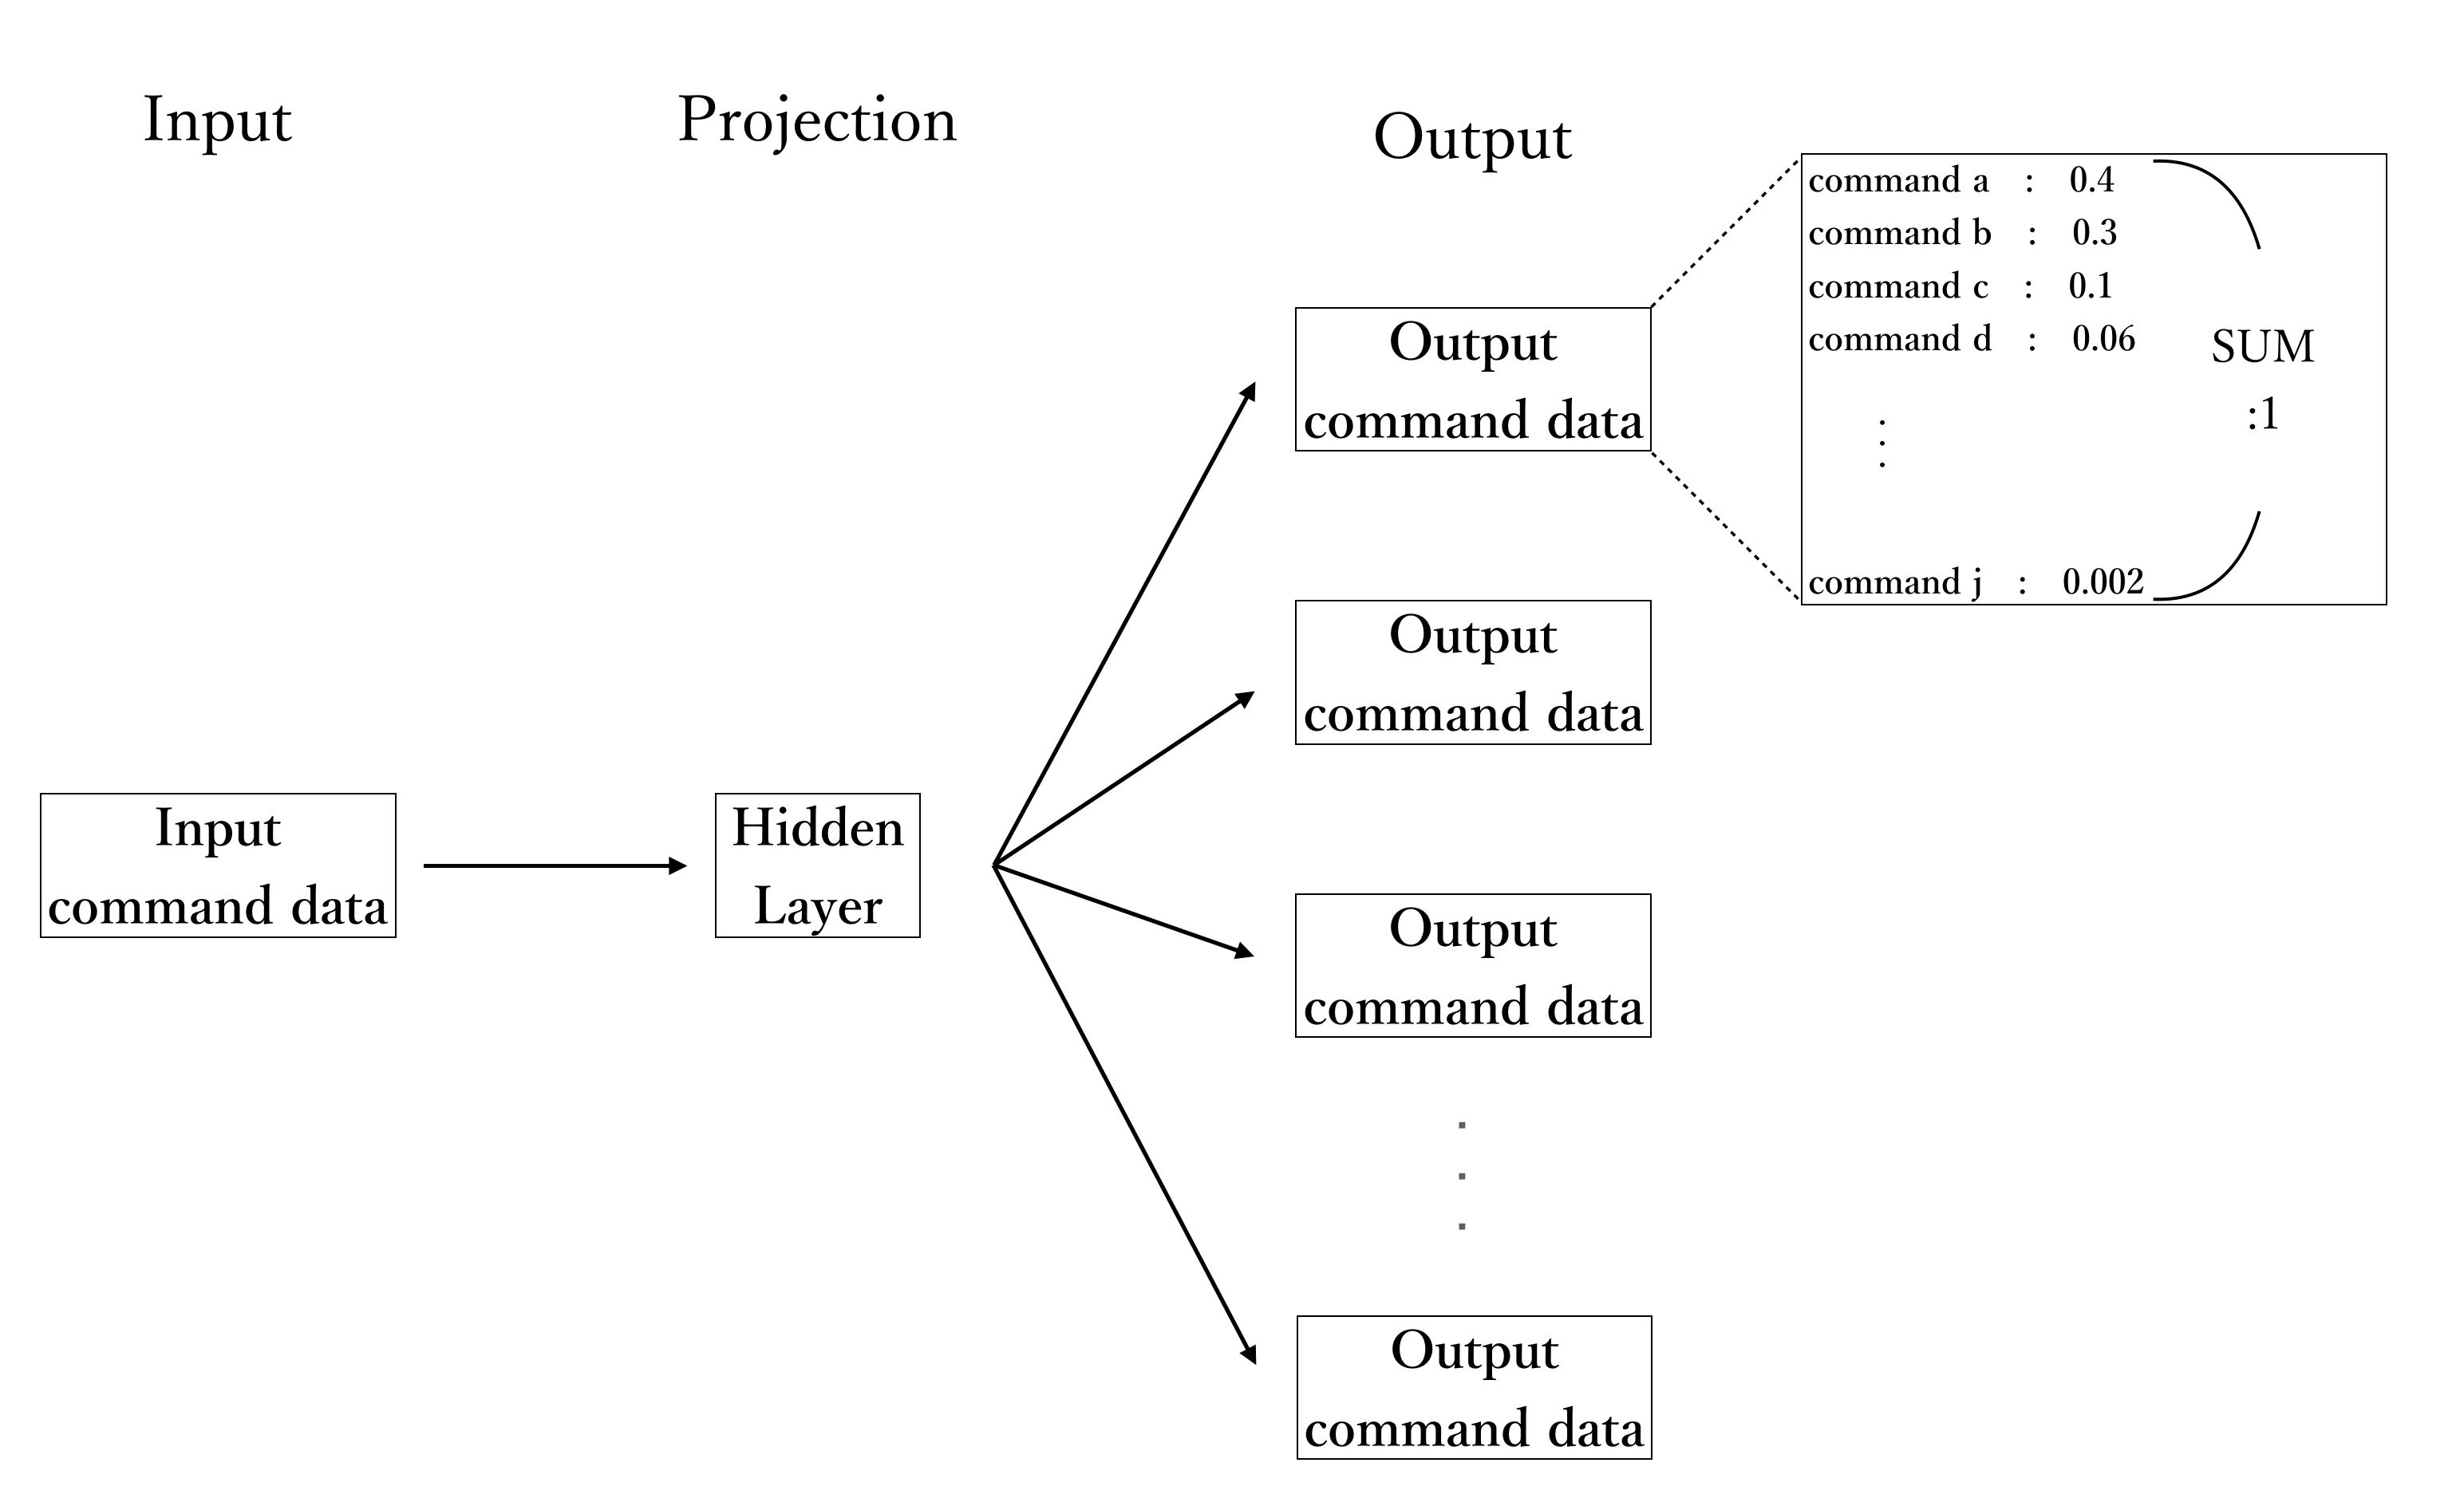
\includegraphics[width=1.0\textwidth]{figures/evalflow.png}
    \caption{評価のフロー\cite{word2vecpaper}\cite{word2vecpaper2}}
    \label{fig:evo}
\end{figure}

このようにして出力された数値を1セッションごとに平均化し,また全てのセッションにおいてもセッションごとに平均化し,全てのセッションの平均化を行うことで,純正の低対話型Honeypotの収集ログと高対話型Honeypotの収集ログとの各々で構築したモデルごとに平均値を算出する.


\subsubsection{コマンド群データのベクトル表現}
\label{eval:CommandVector}

\subsubsection{SSHの低対話型Honeypotの攻撃ログの比較}
\label{eval:CompareLog}


\section{考察}
\label{eval:implkosatu}

%%% Local Variables:
%%% mode: japanese-latex
%%% TeX-master: "./thesis"
%%% End:
